\chapter{Introduction to ECE Linux Programming Environment}
\label{ch_linux_env}

\section{ECE Linux Servers}

There are a group of Linux Ubuntu servers that are open to ECE undergraduate students. The machines are listed at \url{https://ece.uwaterloo.ca/Nexus/arbeau/clients}. To access one of the machines, we recommend using the alias name of \verb+eceubuntu.uwaterloo.ca+, which will redirect you to the most lightly loaded machine at the time of login.

To access these machines from off campus, you can use the \href{https://uwaterloo.ca/information-systems-technology/services/virtual-private-network-vpn}{campus VPN}.
Another way is to first connect to \verb+eceterm.uwaterloo.ca+ and then connect to other Linux servers from there using the ssh command. Note that \verb+eceterm+ should not be used for computing jobs; it is for accessing other Linux servers on campus. Many of the tools you will be using are not supported on eceterm.

\section{Connecting to Linux servers}

A terminal client software that supports secure shell (ssh) will allow you to remotely connect to the Linux servers. MobaXterm is a convenient application that not only supports ssh, but also has a built-in X server that allows you to run Graphical User Interface (GUI) applications from the Linux servers.
\begin{figure}[!htb]
  \centering
  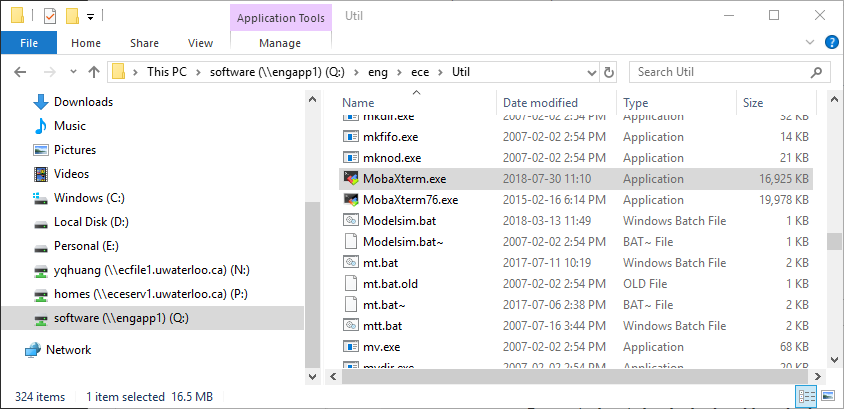
\includegraphics[width=5.5in]{img/lab0/MobaXterm/MobaXterm_Path}
  \caption{MobaXterm Path on ECE Nexus Windows 10 Machines.}
  \label{fig_MobaXterm_Path}
\end{figure}

\begin{figure}[!htb]
  \centering
  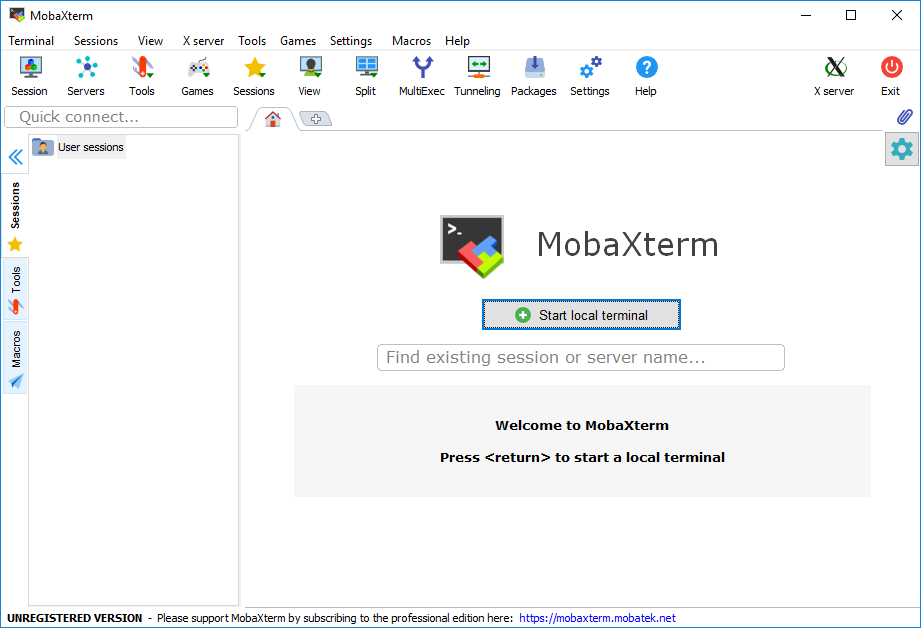
\includegraphics[width=6in]{img/lab0/MobaXterm/MobaXterm_Start_Page}
  \caption{MobaXterm Welcome Page.}
  \label{fig_MobaXterm_Start_Page}
\end{figure}

Use the File Explorer to navigate to the \verb+Q:\eng\ece\Util+ folder, then scroll down until you find the MobaXterm icon and double click it (see Figure \ref{fig_MobaXterm_Path}). The MobaXterm window will pop up. There is a grey rectangular button labelled ``Start local terminal'' in the middle (see Figure \ref{fig_MobaXterm_Start_Page}). Click this button.

Then a terminal session starts. You will need to use the command line \verb+ssh+ command to connect to the eceubuntu server. Use your UW userid and password to login. The syntax of the command is as follows:
%\begin{verbatim}
\begin{lstlisting}[style=bash]
ssh -XY <UWID>@eceubuntu.uwaterloo.ca
\end{lstlisting}
% \end{verbatim}
See Figure \ref{fig_MobaXterm_Login_Password} for reference.
\begin{figure}[!htb]
  \centering
  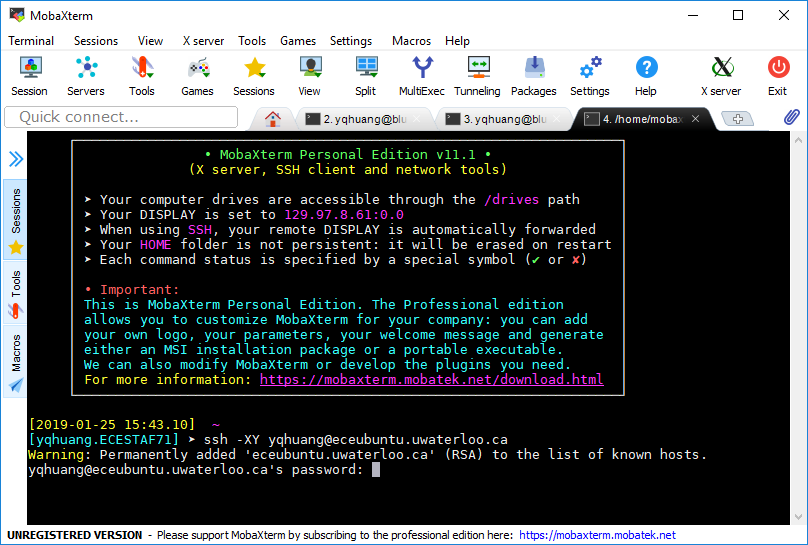
\includegraphics[width=6in]{img/lab0/MobaXterm/MobaXterm_Login_Password}
  \caption{MobaXterm Welcome Page.}
  \label{fig_MobaXterm_Login_Password}
\end{figure}


All your ECE Linux account files are accessible on your P Drive on Nexus machines (See Figure \ref{fig_lab0_P_Drive}). The P Drive is only accessible within the campus network. Mapping the Linux account as a network drive off campus is not supported for security reasons.
\begin{figure}[!htb]
  \centering
  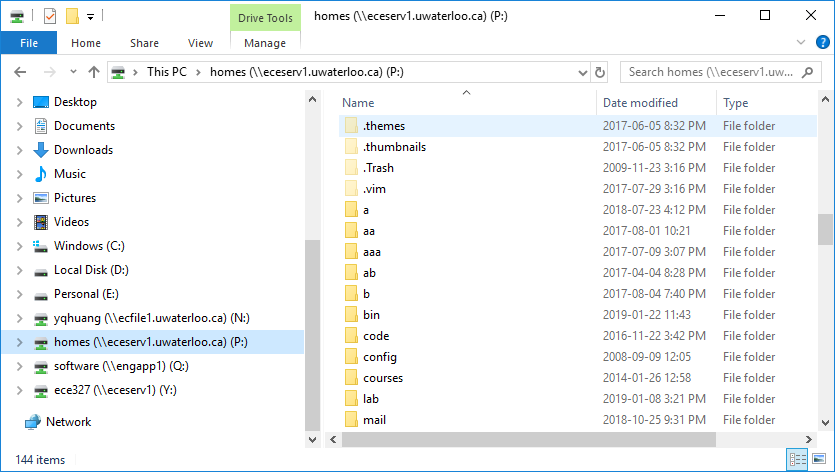
\includegraphics[width=6in]{img/lab0/lab0_P_Drive}
  \caption{Linux files on your P drive, a network mapped drive.}
  \label{fig_lab0_P_Drive}
\end{figure}

\section{Basic Software Development Tools}

%[NOTE: adding a flow chart here]
To develop a program, there are three important steps.
First, a program is created from source code written by a programmer. Second, the source code is compiled into object code, which is a binary file (on Linux, these files have a ".o" extension). A non-trivial project normally contains more than one source file. Each source file is compiled into one object code file and the linker finally links all the object code to generate the final target, which is the executable that you run. The steps of compiling and linking are also known as building a target. It is very rare that the target will run perfectly the first time it is built. Most of time we need to fix defects and bugs in the code (this is the third step). The debugger is a tool to help you identify and fix theses bugs. Table \ref{tb_prog_tools} shows the key steps in programming work flow and example tools provided by a general purpose Linux operating system.

\begin{table}[ht]
\begin{center}
%\footnotesize{
\begin{tabular}{llll}
\hline
Task & Tool & Examples\\ \hline
Editing the source code &    Editor & vi, emacs \\  
Compiling the source code &  Compiler & gcc \\ 
Debugging the program	  &  Debugger & gdb, ddd \\ \hline 
\end{tabular}
%}
\caption{Programming Steps and Tools}
\label{tb_prog_tools}
\end{center}
\end{table}

Most of you are probably more familiar with an Integrated Development Environment (IDE) which integrates all these tools into a single application. Examples of common IDEs are Eclipse and Visual Studio. A different approach is to select a tool for each development step and build your own tool chain. Many seasoned Linux programmers build their own tool chains. A few popular tools are introduced in the following subsections.

\subsection{Editor}

Some editors are better designed to suit programmers' needs than others. The {\em vi} ({\em vim} and {\em gvim} belong to the vi family) and {\em emacs} ({\em xemacs} belongs to emacs family) are the two most popular editors for programming purposes.

%This manual is not meant to teach you how to use these editors. \cite{} are good references to get yourself started with these editors.

Two simple notepad-style editors called {\em pico} and {\em nano} are also available for simple editing jobs. These editors are not designed for programming activity. To use one of them to write your first {\em Hello World} program is fine though. 

After you finish editing the C source code, give the file name an extension of .c. Listing \ref{lst_helloworld} is the source code of printing "Hello World!" to the screen. 

\lstinputlisting[language=C, caption={HelloWorld C source Code}, label=lst_helloworld]{code/linux/HelloWorld/main.c}

\subsection{C Compiler}
The source code then gets fed into a compiler/linker to become an executable program.
The GNU project C and C++ compiler and linker is {\em gcc}. To compile the HelloWorld source code in Listing \ref{lst_helloworld}, type the following command at the prompt:
\begin{lstlisting}[style=bash]
gcc helloworld.c+ 
\end{lstlisting}
You will notice that a new file named \verb+a.out+ is generated.
This is the executable generated from the source code. To run it, type the following command at the prompt and hit Enter.
\begin{lstlisting}[style=bash]
./a.out
\end{lstlisting}
The result is ``Hello World!" appearing on the screen.

You can also instruct the compiler to give the executable another name instead of the default \verb+a.out+. The \verb+-o+ option in gcc allows you to give the executable a name. For example, the following command will generate an executable named ``\verb+helloworld.out+".
\begin{lstlisting}[style=bash]
gcc helloworld.c -o helloworld.out
\end{lstlisting}
although there is no requirement that the name ends in \verb+.out+.
\subsection{Debugger}
The GNU debugger gdb is a command line debugger. Many GUI (i.e. visual)  debuggers uses gdb as their back-end engine. One popular GNU GUI debugger is {\em ddd}. It has a powerful data display functionality. 

GDB needs to read debugging information from the binary in order to be able to help you to debug the code. The \verb+-g+ option in gcc tells the compiler to produce such debugging information in the generated executable. In order to use gdb to debug our simple HelloWorld program, we need to compile it with the following command:
\begin{lstlisting}[style=bash]
gcc -g helloworld.c -o helloworld.out
\end{lstlisting}

The following command calls gdb to debug helloworld.out 
\begin{lstlisting}[style=bash]
gdb helloworld.out 
\end{lstlisting}
This starts a gdb session. At the \verb+(gdb)+ prompt, you can issue gdb commands such as \verb+b main+ to set up a break point at the entry point of the main function. The \verb+l+ command lists source code. The \verb+n+ command steps to the next statement in the same function. The \verb+s+ command steps into a function. The \verb+p+ command prints a variable value provided you supply the name of the variable. Type \verb+h+ to see more gdb commands.


Compared to the gdb command line interface, the ddd GUI interface is more user friendly and easy to use. To start a ddd session,
type the command
\begin{lstlisting}[style=bash]
ddd 
\end{lstlisting}
and click File $\rightarrow$ Open Program to open an executable such as helloworld.out. You will then see the gdb console in the bottom window with the source code window above it. You can see the values of variables in the data window, which is above the source code window. Select View to toggle all of these windows. 

A good gdb/ddd tutorial can be found at \url{https://www.cs.swarthmore.edu/~newhall/unixhelp/howto_gdb.php}. Pay special attention to the section on how to troubleshoot segmentation fault problems.
\section{More on Development Tools}

For any non-trivial software project, you normally have multiple source code files. Developers need tools to manage the project build process. Also projects are normally done by several developers. A version control tool is also needed.

\subsection{How to Automate Builds}

Make is a utility to automate the build process. Compilation is a cpu-intensive job and one only wants to re-compile the files that have been changed when you build a target instead of re-compiling all source file regardless. 
The \verb+make+ utility uses a Makefile to specify the dependency of object files and automatically recompiles files that have been modified after the last target has been built. 

In a Makefile, you specify the targets to be built, what prerequisites the target depends on, and what commands are used to build the target. These are the {\em rules} contained in a Makefile. Makefiles have their own syntax.
The general form of a Makefile rule is:
\begin{lstlisting}[style=makefile]
target ...: prerequisites ... 
        recipe
        ...	
        ...	
\end{lstlisting}
One important note is that each recipe line starts with a TAB key rather than white spaces. To build a target, use the command \verb+make+ followed by the target name or omit the target name to default to the first target in the Makefile. For example
\begin{lstlisting}[style=bash]
make
\end{lstlisting}
will build your lab starter code.

Listing \ref{lst_makefile_hello} is our first attempt to write a very simple Makefile.

\lstinputlisting[
    language=make, 
    caption={Hello World Makefile: First Attempt}, 
    style=makefile,
    label=lst_makefile_hello
]{code/linux/HelloWorld/Makefile1}
The following command will generate the \verb+helloworld.out+ executable file.
\begin{lstlisting}[style=bash]
make helloworld.out
\end{lstlisting}

Our second attempt is to break the single line gcc command into two steps. The first is to {\em compile} the source code into an object code .o file. The second is to {\em link} the object code to one final executable binary. 
Listing \ref{lst_makefile_hello2} is our second attempted  version of Makefile.

\lstinputlisting[
    language=make, 
    caption={Hello World Makefile: Second Attempt}, 
    style=makefile,
    label=lst_makefile_hello2
]{code/linux/HelloWorld/Makefile2}

When a project contains multiple files, separating the compilation and linking stages gives a clear dependency relationship among code. Assume that we now need to build a project that contains two source files \verb+src1.c+ and \verb+src2.c+ and we want the final executable to be named \verb+app.out+.
Listing \ref{lst_makefile3} is a typical example Makefile that is closer to what you will see in the real world.
\lstinputlisting[
    language=make, 
    caption={A More Real Makefile: First Attempt}, 
    style=makefile,
    label=lst_makefile3
]{code/linux/HelloWorld/Makefile3}
We have also added a target named {\em clean} so that \verb+make clean+ will clean the build.

So far we have seen that the Makefile contains {\em explicit rules}. A Makefile can also contain {\em implicit rules}, {\em variable definitions}, {\em directives} and
{\em comments}. 
Listing \ref{lst_makefile4} is a Makefile that is used in the real world.
\lstinputlisting[
    language=make, 
    numbers=left,
    numberstyle=\tiny,
    stepnumber=1,
    numbersep=5pt,
    caption={A Real World Makefile}, 
    style=makefile,
    label=lst_makefile4
]{code/linux/HelloWorld/Makefile4}
Line $1$ is a comment. Lines $2-7$ are variable definitions. Line $12$ is an implicit rule to generate a .o file for each .c file. 
See \url{http://www.gnu.org/software/make/manual/make.html} to explore more about makefiles.

\subsection{Version Control Software}
We use the Git version control software. It is installed both on the Linux servers and the Nexus Windows machines. If you decide to use GitHub to host your repository, please make sure it is a {\em private} one. Go to \url{http://github.com/edu} to see how to obtain five private repositories for two years on GitHub for free. 
%This [] is a good reference on how to use Git and Dropbox together to create private repositories.

%Table \ref{} lists some frequently used git commands.

\subsection{Integrated Development Environment}
Eclipse with the C/C++ Plug-in has been installed on all ECE Linux servers. Type the following command to bring up the Eclipse frontend.
\begin{lstlisting}[style=bash]
/opt/eclipse64/eclipse
\end{lstlisting}
This Eclipse is not the same as the default Eclipse under the \verb+/usr/bin+ directory. You may find running Eclipse over a network performs poorly at home though. It depends on how fast your network speed is. 

If you have a Linux operating system installed on your own personal computer, then you can download Eclipse with the C/C++ plugin from the Eclipse web site and then run it from your own local computer. However you should always make sure that your program will also work on the eceubuntu machines, since that is the environment TAs will be using to test your code.

\section{Man Page}
Linux provides manual pages. You can use the command \verb+man+ followed by the specific command or function you are interested in to obtain detailed information. 

Manual pages are grouped into sections. We list frequently used sections here: 
\begin{itemize}
\item Section 1 contains user commands
\item Section 2 contains system calls
\item Section 3 contains library functions
\item Section 7 covers conventions and miscellany
\end{itemize}

To specify which section you want to see, provide the section number after the \verb+man+ command. For example,
\begin{lstlisting}[style=bash]
man 2 stat
\end{lstlisting}
shows the system call \verb+stat+ man page. If you omit the \verb+2+ in the command, then it will return the command \verb+stat+ man page from section 1 of the manual.

You can also use \verb+man -k+  or \verb+apropos+ followed by a string to obtain a list of man pages that contain that string, using the Whatis database. You can run \verb+man whatis+ to see more details about \verb+whatis+.

%%% Local Variables:
%%% mode: latex
%%% TeX-master: "main_book"
%%% End:
